\section{Oferecimento} 

\textbf{Em nome do Pai, do Filho e do Espírito Santo. Amém.}

Uno-me a todos os Santos que estão no Céu, a todos os justos que estão sobre a Terra, a todas as almas fiéis que estão neste lugar. Uno-me a Vós, meu Jesus, para louvar dignamente Vossa Santa Mãe, e louvar-Vos a vós nela e por ela. Renuncio a todas as distrações que me vierem durante este Terço que quero recitar com modéstia, atenção e devoção como se fosse o último de minha vida. Nós Vos oferecemos, Trindade Santíssima, este Credo, para honrar os mistérios todos de nossa Fé; este Pater e estas três Ave-Marias, para honrar a unidade de Vossa essência e a Trindade de Vossas pessoas. Pedimo-Vos uma fé viva, uma esperança firme e uma caridade ardente. Rezamos também pelas santas almas no purgatório, pelos sacerdotes e religiosos consagrados, pelas vocações e pelo Santo Padre, o papa \textbf{[nome do papa]}. 
Rezamos também pelas seguintes intenções anexas… \textbf{[mencionar as intenções.]}


\begin{center}
  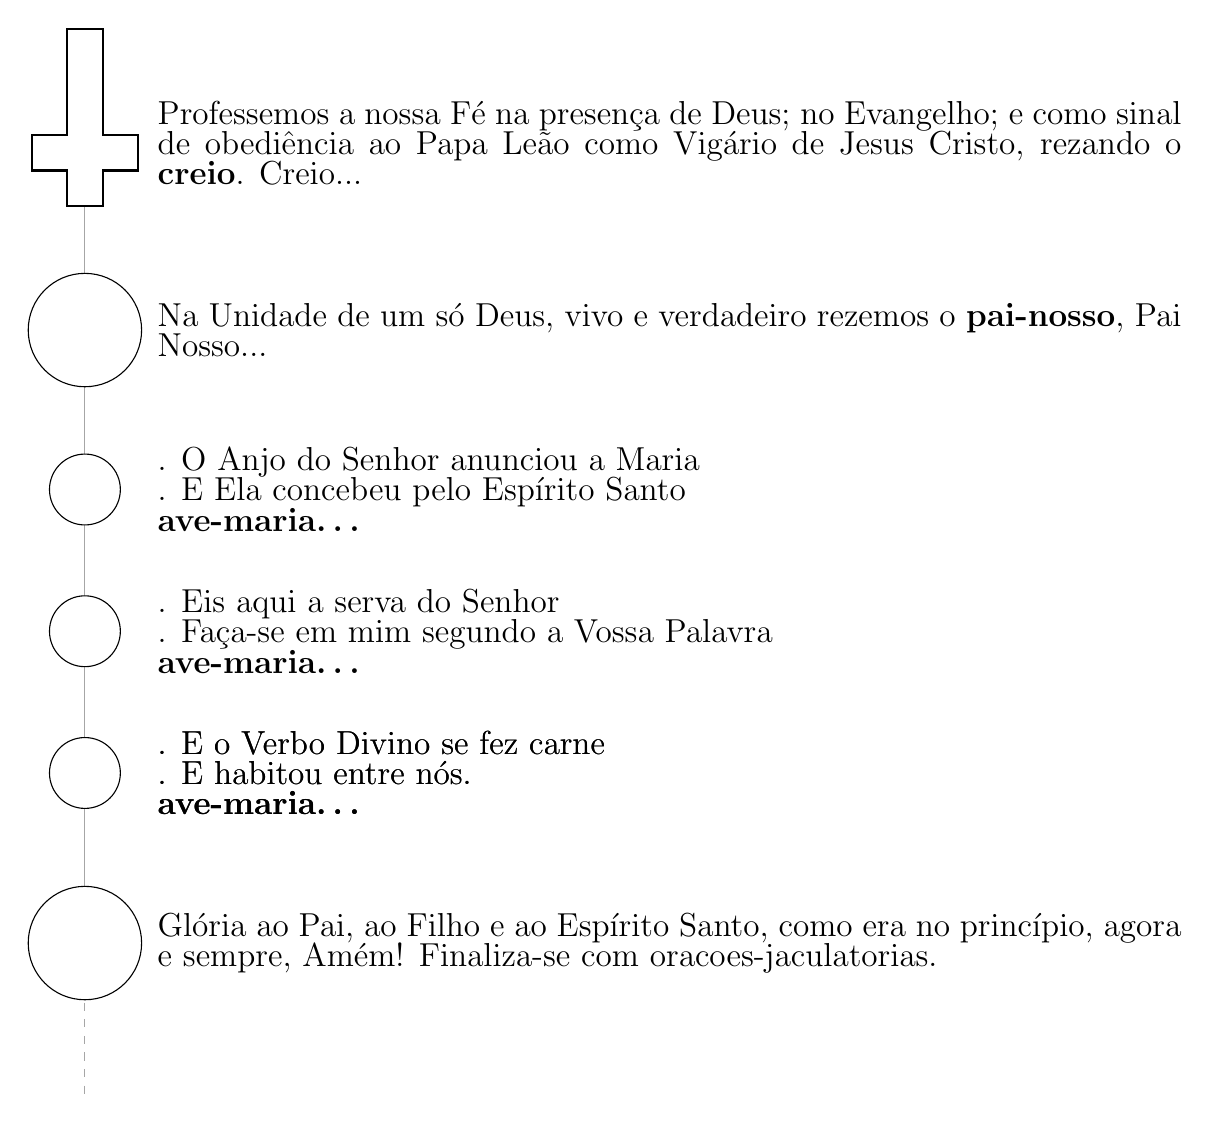
\begin{tikzpicture}[
    scale=1.8,
  rotate=180,
  every node/.style={anchor=west, align=justify, text width=13cm, font=\fontsize{12}{11}\selectfont},
    ]

  \coordinate (center) at (0,-.2);
  \coordinate (cross-origin) at (0,-5);

  % linha da cruz
  \draw[gray!70] (cross-origin) -- (center);
  \draw[dashed, gray!70] (center) -- ++(0,1.5);

  % contas

  %% jaculatórias
  \draw[fill=white] (center) ++ (0,0.4) coordinate(gloria) circle (0.4);

  \draw[fill=white] (0,-1) coordinate(conta1) circle (0.25)
  ++(0, -1) coordinate(conta2) circle (0.25) 
  ++(0, -1) coordinate (conta3) circle (0.25) 
  ++(0, -1.125) coordinate(conta4) circle (0.4);

  % cruz
  \draw[black, thick] (cross-origin) -- ++(0.125, 0) -- ++(0,-.25) -- ++(.25,0) -- ++(0,-.25) -- ++ (-.25,0) -- ++(0, -.75) -- ++(-.25,0) -- ++ (0,.75) --++ (-.25,0) -- ++ (0,.25) -- ++ (.25,0) -- ++ (0,.25) -- (cross-origin);

  \node at (cross-origin) [above=.8cm , right=0.8cm] {
Professemos a nossa Fé na presença de Deus; no Evangelho; e como sinal de obediência ao Papa Leão como Vigário de Jesus Cristo, rezando o \textbf{\nameref{creio}}. Creio...
  };

  \node at (conta4) [right=0.8cm] {Na Unidade de um só Deus, vivo e verdadeiro rezemos o \textbf{\nameref{pai-nosso}}, Pai Nosso...};

  \node at (conta3) [, right=0.8cm] {
    \versicle. O Anjo do Senhor anunciou a Maria \\
    \response. E Ela concebeu pelo Espírito Santo\\
    \textbf{\nameref{ave-maria}…}
  };
  \node at (conta2) [, right=0.8cm] {
    \versicle. Eis aqui a serva do Senhor\\
    \response. Faça-se em mim segundo a Vossa Palavra\\
    \textbf{\nameref{ave-maria}…}
  };

  \node at (conta1) [, right=0.8cm] {
    \versicle. E o Verbo Divino se fez carne\\
    \response. E habitou entre nós.\\
    \textbf{\nameref{ave-maria}…}
  };

  \node at (conta1) [, right=0.8cm] {
    \versicle. E o Verbo Divino se fez carne\\
    \response. E habitou entre nós.\\
    \textbf{\nameref{ave-maria}…}
  };

  \node at (gloria) [, right=0.8cm] {
    Glória ao Pai, ao Filho e ao Espírito Santo, como era no princípio, agora e sempre, Amém! Finaliza-se com \nameref{oracoes-jaculatorias}.
  };

  \end{tikzpicture}
\end{center}

\newpage
